\section{Introduction}

The market for mobile applications is booming. In 2015, global application downloads are estimated to be $179$ billion \cite{downloads}, generating $\$45$ billion revenues \cite{revenue} and involving $5.5$ million developers \cite{developer}. To compete for market share and profits, application developers are motivated to provide quality service with reduced cost.

Backend provisioning is one of the fundamental concerns for developers, as all user requests from the frontend of an application need to be handled by the backend. Developers can either use Mobile-backend-as-a-Service (MBaaS) or build their own backends on cloud platforms (such as Amazon EC2). In the former case, developers can directly enjoy backend services offered by MBaaS providers, who charge fees based on the number of requests sent to the MBaaS backend.  In the latter case, developers can construct their backends using instances, and pay for their usage.

One of the biggest challenges facing backend provisioning is a mismatch between timescales of request demand variance and backend resource availability. The rate at which user requests arrive at the backend varies from second to second, but developers can neither change the MBaaS service plan nor adjust instance configurations at such a fine granularity of time. Though Amazon EC2 also provides auto-scaling mechanisms, it requires developers to determine how many instances to add or reduce, and it takes time to boot up or shut down computers. Rather than trying to let the backend capacity closely \emph{track} the demand profile, which is difficult or even impossible to realize, we explore a new way of backend provisioning. We \emph{smooth} the demand profile by redistributing delay-tolerant requests and prioritizing delay-sensitive requests, which potentially lightens the burdens on the backend and saves money for developers.

\begin{figure}[t]
	\centering
	\hspace{-0.4cm}
	\begin{minipage}[t]{1.7in}
		\centering
		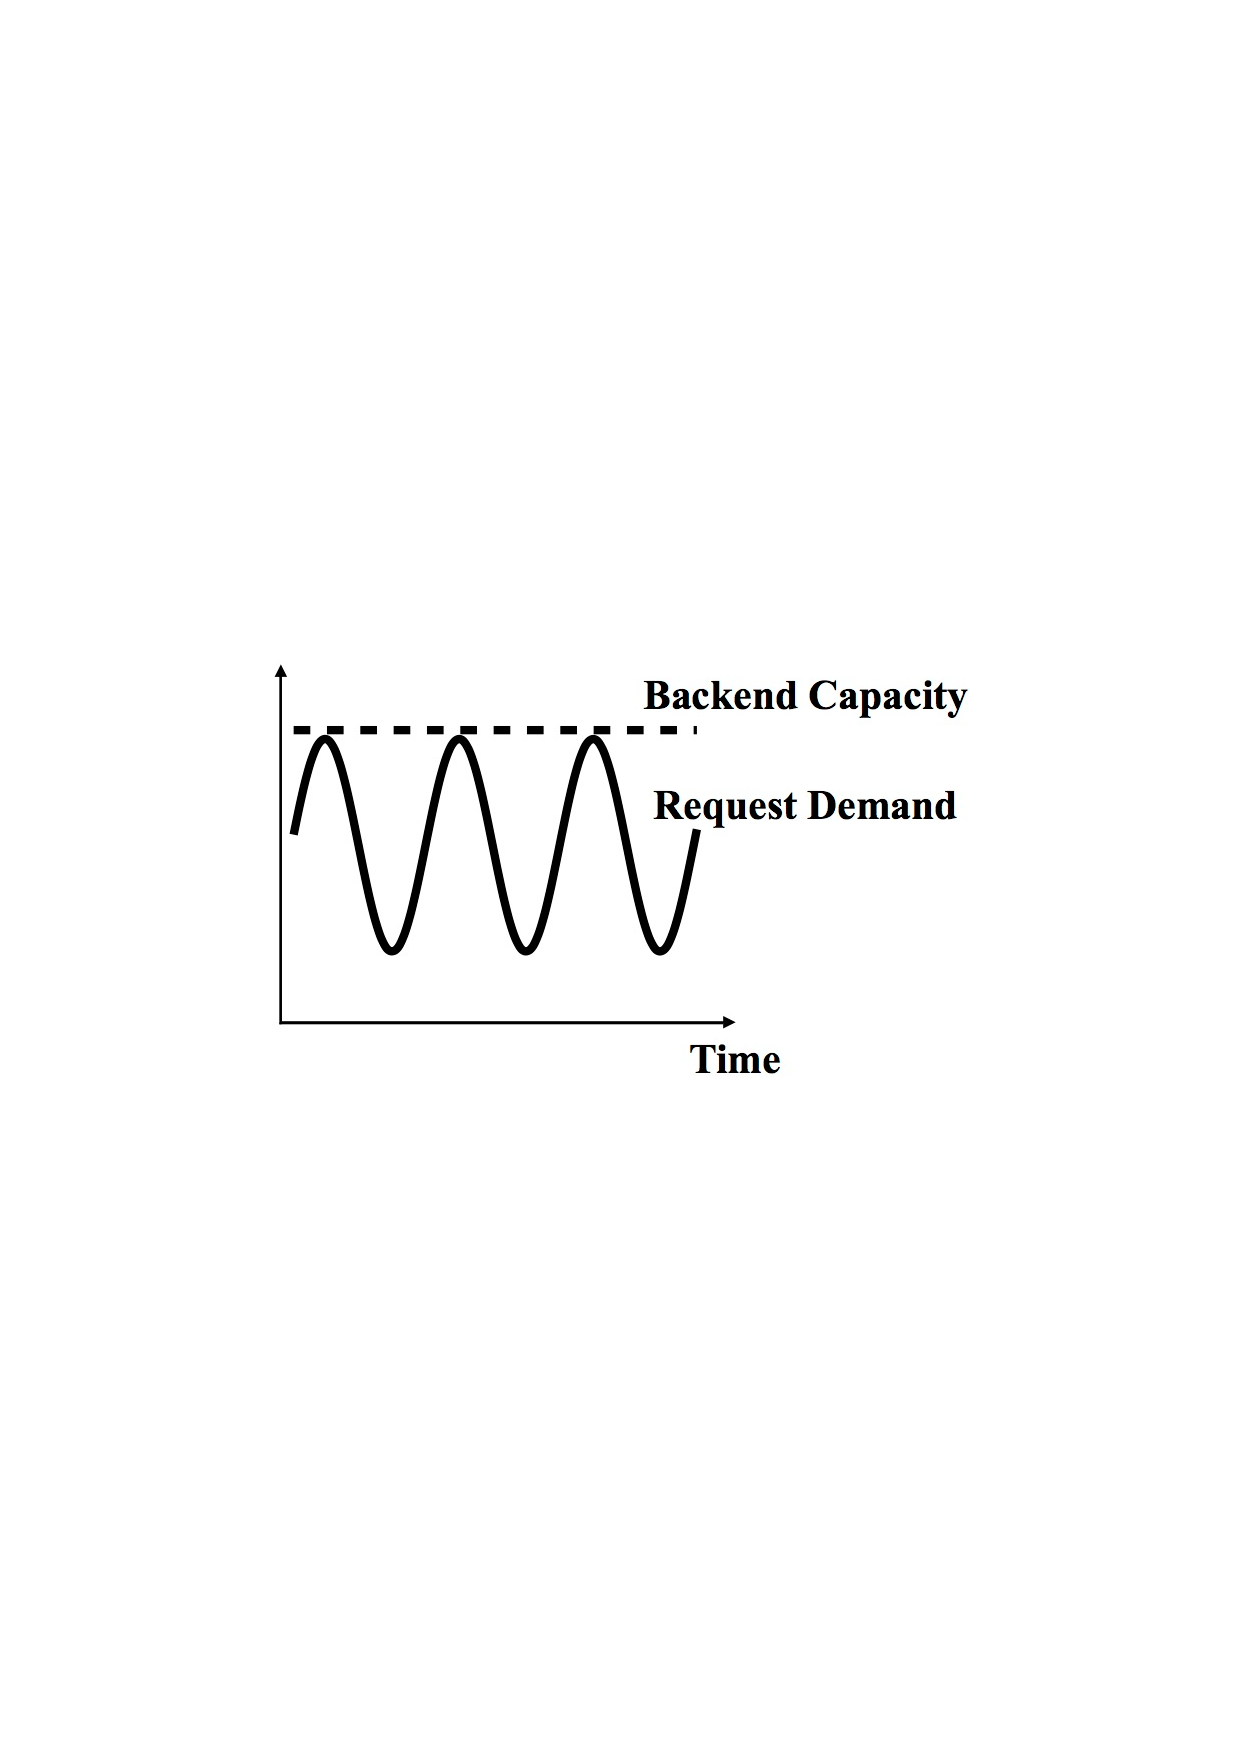
\includegraphics[trim=45mm 110mm 45mm 110mm, clip,width=1.7in]{figs/intro1}\\
		\centerline{(a) Provisioning for}
		\centerline{peak demand}
	\end{minipage}
	\hspace{-0.1cm}
	\begin{minipage}[t]{1.8in}
		\centering
		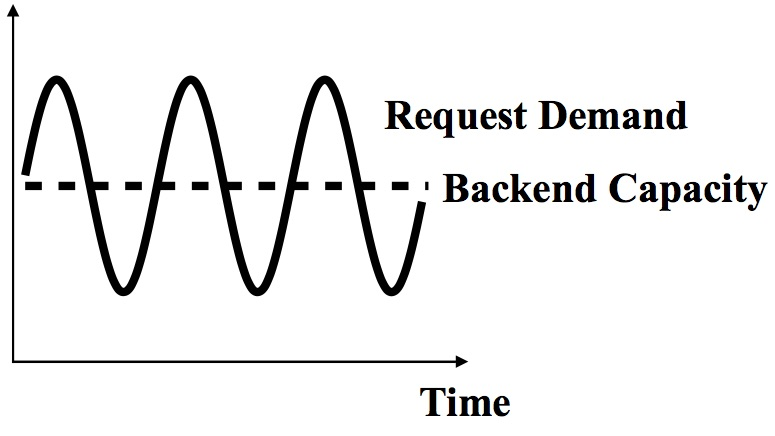
\includegraphics[trim=40mm 110mm 40mm 110mm, clip,width=1.8in]{figs/intro2}\\
		\centerline{(b) Provisioning for}
		\centerline{average demand}
	\end{minipage}
	\hspace{-0.cm}
	\begin{minipage}[t]{1.8in}
		\centering
	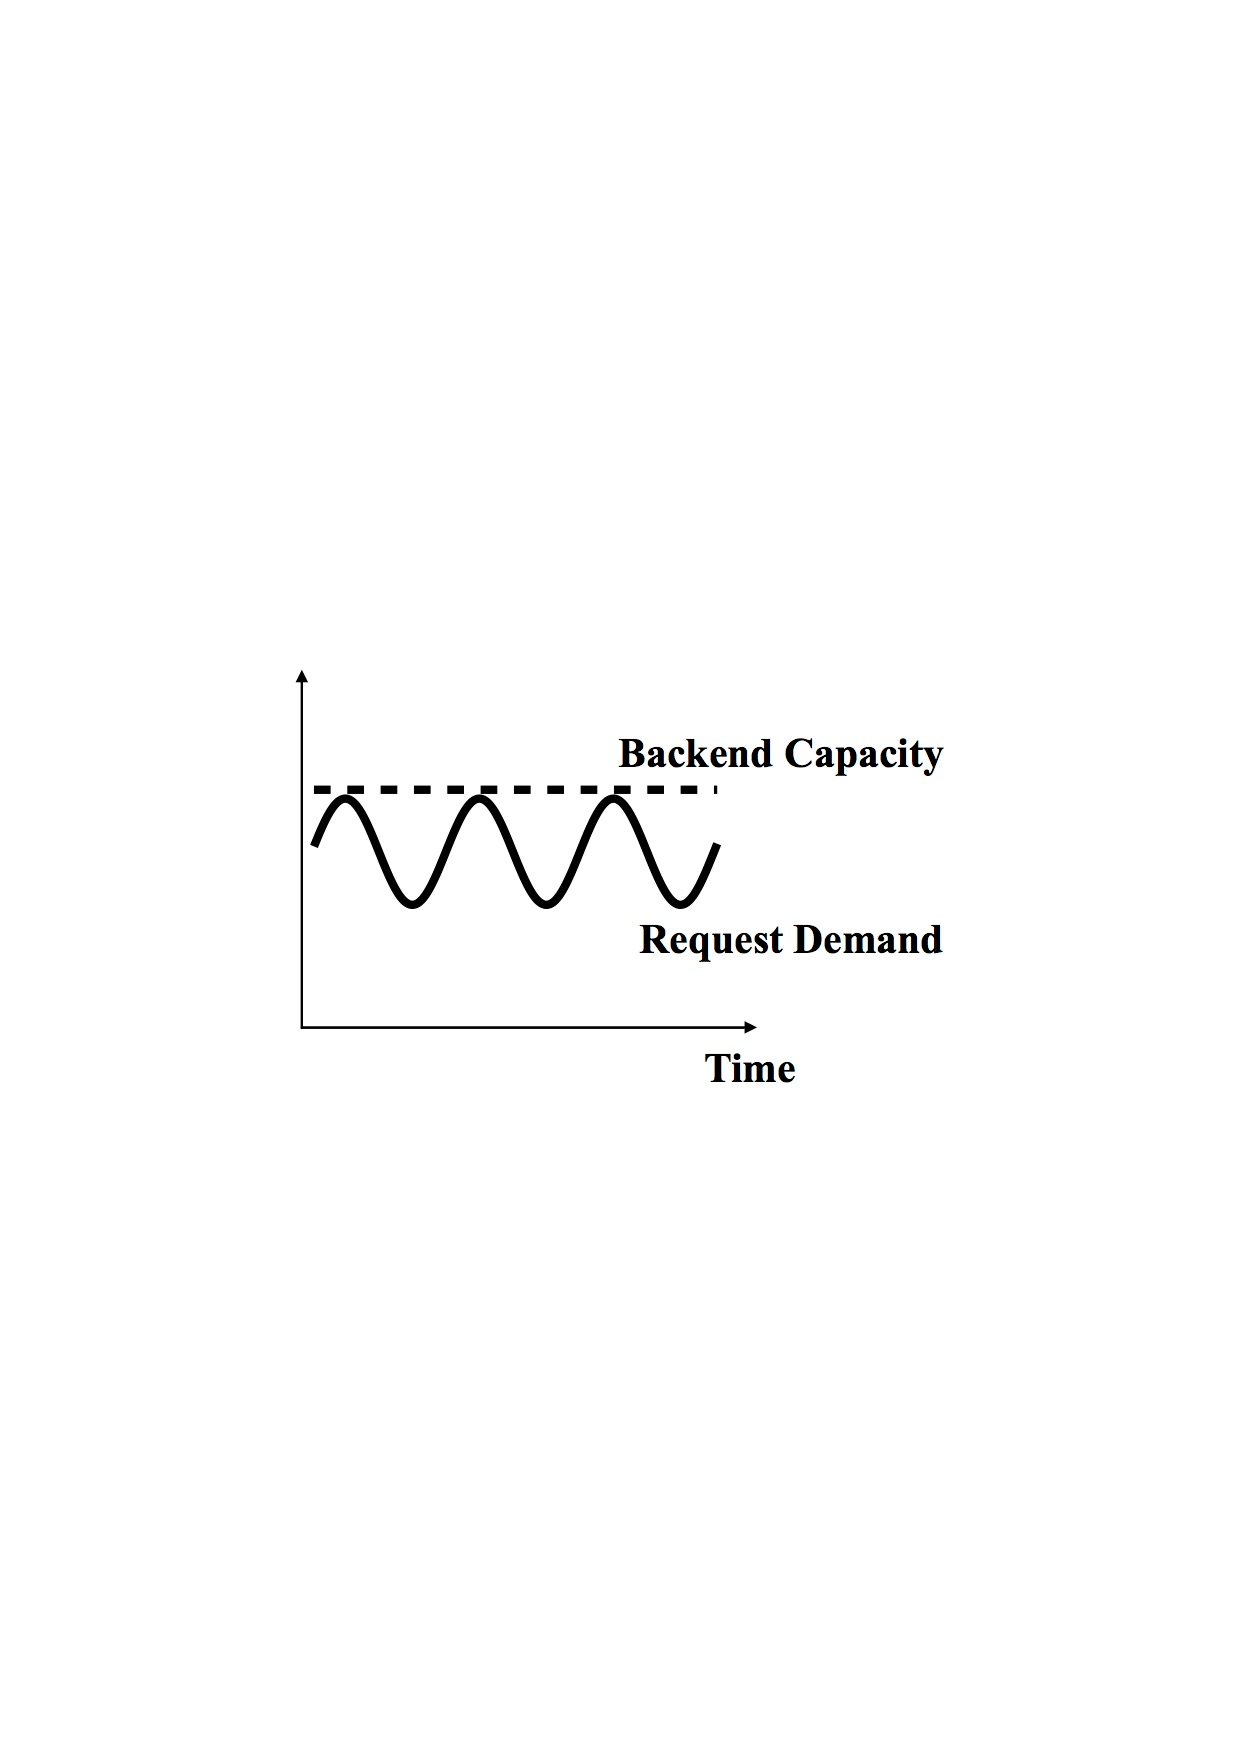
\includegraphics[trim=50mm 110mm 45mm 110mm, clip,width=1.8in]{figs/intro3}\\
		\centerline{(c) Clockwork}
	\end{minipage}
	\caption{Backend provisioning comparison.} \label{fig:intro}
\end{figure}

To achieve such a goal, we present Clockwork, a third-party cloud service designed to help developers manage backend provisioning. Clockwork features a two-tier architecture: backend capacity planning on a long timescale, and rate-based request scheduling on a short timescale. Both tiers are indispensable in helping developers maintain a sufficient and cost-effective backend. As shown in Fig.~\ref{fig:intro}(a), if the backend capacity caters to the peak demand to avoid any performance degradation, there will be a considerable wastage of resources and money. Nevertheless, if the backend capacity falls short of the peak demand, as shown in Fig.~\ref{fig:intro}(b), some requests will have to be dropped or experience unacceptably long processing times. In comparison, Clockwork schedules requests according  to delay tolerance, as shown in Fig.~\ref{fig:intro}(c), thus flattening the request demand and slashing the required backend capacity.


There are several challenges facing the implementation of Clockwork. To plan for the long-term backend capacity, it is crucial to have an accurate prediction of the future request demand. There is a wide variety of machine learning algorithms for data prediction, each of which has their advantages and disadvantages. We compare the prediction accuracy and training time of four machine learning algorithms (Section \ref{sec:predict}). It is shown that deep learning algorithms, including convolutional neural networks and deep belief networks, yield better prediction results but require a much longer time to train than simpler machine learning algorithms, such as logistic regression and multilayer perceptron. With the estimated future demand, the Clockwork derives the optimal backend capacity that minimizes developer's cost, while conforming to the constraint on request delay  (Section \ref{sec:plan}).

Given the long-term capacity, to ensure that the backend is not overwhelmed by instant request demand, we adopt a rate-based resource allocation strategy (Section \ref{sec:rateall}). Clockwork centrally assigns rates to users based on the quantity and delay tolerance of their requests, then individual users autonomously schedule their own requests. We build a network utility maximization (NUM) model to decide the rate allocation, which is proved to be fair and Pareto-optimal.



We have implemented the server-side of Clockwork using the Amazon Web Service (AWS), and the client-side of Clockwork on iOS-based mobile devices. We present the implementation details (Section \ref{sec:implementation}) and evaluate the performance of Clockwork by a small-scale pilot experiment and a large-scale simulation (Section \ref{sec:experiment}). The results show that Clockwork can help developers substantially cut down the backend cost, as well as improve the backend utilization.











